\chapter{द्रव्यमान और आयतन}\label{ch:g6:mass-and-volume}

बोतल में कितनी शिकंजी समाती है, और बोतलों की पेटी कितनी भारी है? ये
दो अलग सवाल हैं --- जगह और पदार्थ --- जिन्हें रोज़ की बातचीत ख़ुशी-ख़ुशी
``बड़ा'' नाम के एक ही शब्द में उलझा देती है। विज्ञान उन्हें सुलझा देता
है: किसी चीज़ के घेरे हुए स्थान के लिए \omterm{def:g6:mass-and-volume:volume}{आयतन}, और उसमें भरे पदार्थ के
लिए \omterm{def:g3:measuring-mass:mass}{द्रव्यमान}। दूसरा मापने में तुम पुराने खिलाड़ी हो; आज हम पहला \omterm{def:g6:measurement-in-science:measuring}{मापना}
सीखेंगे --- यहाँ तक कि उस कंकड़ का भी, जिसका आकार किसी रूलर को कभी
प्यारा नहीं लगेगा।

\section{आयतन: घेरा हुआ स्थान}

\begin{definition}[आयतन]\label{def:g6:mass-and-volume:volume}
किसी चीज़ का \emph{आयतन}\index{आयतन} उतना स्थान है जितना वह घेरती है।
\omterm{def:g3:solids-liquids-gases:solid}{ठोस}, \omterm{def:g3:solids-liquids-gases:liquid}{द्रव} और गैसें --- सबका आयतन होता है: ईंट अपनी जगह घेरती है,
शिकंजी बोतल का भीतरी हिस्सा, और \omterm{def:g2:air-around-us:air}{हवा} बाक़ी बचा हुआ। आयतन \emph{घन
सेंटीमीटर}\index{घन सेंटीमीटर} (\unit{cm^3}) में मापा जाता है ---
यानी उस नन्हे घन का स्थान जिसका हर किनारा एक \omterm{def:g2:measuring-length:units}{सेंटीमीटर} का हो --- और
\emph{लीटर}\index{लीटर} (\unit{L}) में भी।
\end{definition}

\begin{proposition}[घनों में लीटर]\label{prop:g6:mass-and-volume:litre}
\omterm{def:g6:mass-and-volume:volume}{आयतन} के दोनों मात्रक-कुनबे असल में एक ही कुनबा हैं:
\[
\qty{1}{L} = \qty{1000}{cm^3},
\qquad
\qty{1}{mL} = \qty{1}{cm^3}.
\]
एक \omterm{def:g6:mass-and-volume:volume}{लीटर} ठीक उतना स्थान है जितना उस घन के भीतर होता है जिसका हर किनारा
दस \omterm{def:g2:measuring-length:units}{सेंटीमीटर} का हो: $10 \times 10 \times 10 = 1000$ नन्हे घन।
\end{proposition}

\begin{omfigure}
\begin{tikzpicture}[scale=0.85]
  \draw[thick] (0,0) rectangle (3,3);
  \draw[thick] (0,3) -- (0.9,3.75) -- (3.9,3.75) -- (3,3);
  \draw[thick] (3.9,3.75) -- (3.9,0.75) -- (3,0);
  \foreach \i in {1,...,9} {
    \draw[very thin] (0,0.3*\i) -- (3,0.3*\i);
    \draw[very thin] (0.3*\i,0) -- (0.3*\i,3);
    \draw[very thin] (0.3*\i,3) -- (0.3*\i+0.9,3.75);
    \draw[very thin] (3,0.3*\i) -- (3.9,0.3*\i+0.75);
    \draw[very thin] (0.09*\i,3+0.075*\i) -- (3+0.09*\i,3+0.075*\i);
    \draw[very thin] (3+0.09*\i,0.075*\i) -- (3+0.09*\i,3+0.075*\i);
  }
  \draw[thick, fill=omDef, fill opacity=0.6]
    (0,2.7) rectangle (0.3,3);
  \node[right, font=\small] at (4.6,3.0)
    {बड़ा घन: हर किनारा \qty{10}{cm}};
  \node[right, font=\small] at (4.6,2.2)
    {$10 \times 10 \times 10 = 1000$ नन्हे घन};
  \node[right, font=\small] at (4.6,1.4)
    {हर नन्हा घन: \qty{1}{cm^3}};
  \node[right, font=\small, omDef] at (4.6,0.6)
    {पूरा: $\qty{1000}{cm^3} = \qty{1}{L}$};
\end{tikzpicture}

{\small एक \omterm{def:g6:mass-and-volume:volume}{लीटर}, खोलकर दिखाया गया: \omterm{def:g2:measuring-length:units}{सेंटीमीटर} वाले हज़ार घन, दस-दस के
तीन तलों में चुने हुए।}
\end{omfigure}

\begin{example}[याद रखने लायक आयतन]\label{ex:g6:mass-and-volume:byheart}
एक छोटी चम्मच में लगभग \qty{5}{mL} आता है; पीने के गिलास में लगभग
\qty{25}{cL}, यानी चौथाई \omterm{def:g6:mass-and-volume:volume}{लीटर}; दूध के डिब्बे में \qty{1}{L}; नहाने के
टब में लगभग \qty{150}{L}; चीनी की एक डली लगभग \qty{3}{cm^3} घेरती
है; और पासा लगभग \qty{4}{cm^3}। ऐसे लंगर हर मापन के परखने वाले क़दम
को संभव बनाते हैं।
\end{example}

\section{द्रवों को मापना}

\begin{method}[मापक बेलन पढ़ना]\label{met:g6:mass-and-volume:cylinder}
प्रयोगशाला का जग \emph{मापक बेलन} है: ऊँचा, पतला, और बारीकी से
अंशांकित।
\begin{enumerate}
  \item बेलन को समतल मेज़ पर रखो --- उसे कभी हाथ में पकड़कर मत
        पढ़ो;
  \item हर मापनी की तरह एक पायदान का मान निकालो;
  \item अपनी आँख \omterm{def:g3:solids-liquids-gases:liquid}{द्रव} की सतह के बराबर लाओ: वह सतह सपाट नहीं बल्कि
        ज़रा-सी मुड़ी होती है --- यही
        \emph{नवचंद्रक}\index{नवचंद्रक} है --- जो काँच की दीवारों
        पर थोड़ा ऊपर चढ़ जाती है;
  \item पाठ उस मोड़ के \emph{सबसे नीचे} वाले हिस्से पर, सीधे सामने
        से लो।
\end{enumerate}
आँख बहुत ऊँची या बहुत नीची हो, तो वह मोड़ तुमसे एक-दो पायदान का झूठ
बोल देता है --- यानी तिरछी नज़र वाली ग़लती अपने पसंदीदा भेस में।
\end{method}

\begin{omfigure}
\begin{tikzpicture}[scale=0.85]
  \draw[thick] (1.0,0) -- (1.0,4.2) (3.0,0) -- (3.0,4.2);
  \draw[thick] (1.0,0) -- (3.0,0);
  \fill[omDef, opacity=0.2] (1.0,0.05) rectangle (3.0,2.6);
  \draw[omDef, very thick]
    (1.0,2.75) .. controls (1.6,2.55) and (2.4,2.55) .. (3.0,2.75);
  \foreach \y/\l in {0.6/10, 1.4/20, 2.2/30, 3.0/40, 3.8/50} {
    \draw (3.0,\y) -- (3.25,\y);
    \node[right, font=\footnotesize] at (3.3,\y) {\l};
  }
  \draw[-Stealth, omThm, thick] (6.3,2.6) -- (2.2,2.6);
  \node[right, font=\small, omThm] at (6.4,2.6)
    {मोड़ के सबसे नीचे पढ़ो: \qty{28}{mL}};
  \node[below, font=\small] at (2.0,-0.35)
    {आँख सतह के बराबर, बेलन मेज़ पर};
\end{tikzpicture}

{\small \omterm{met:g6:mass-and-volume:cylinder}{नवचंद्रक}: \omterm{def:g3:solids-liquids-gases:liquid}{द्रव} काँच पर थोड़ा ऊपर चढ़ जाते हैं। ईमानदार पाठ
मोड़ के सबसे नीचे वाले हिस्से पर है, आँख उसी के बराबर।}
\end{omfigure}

\begin{omfigure}
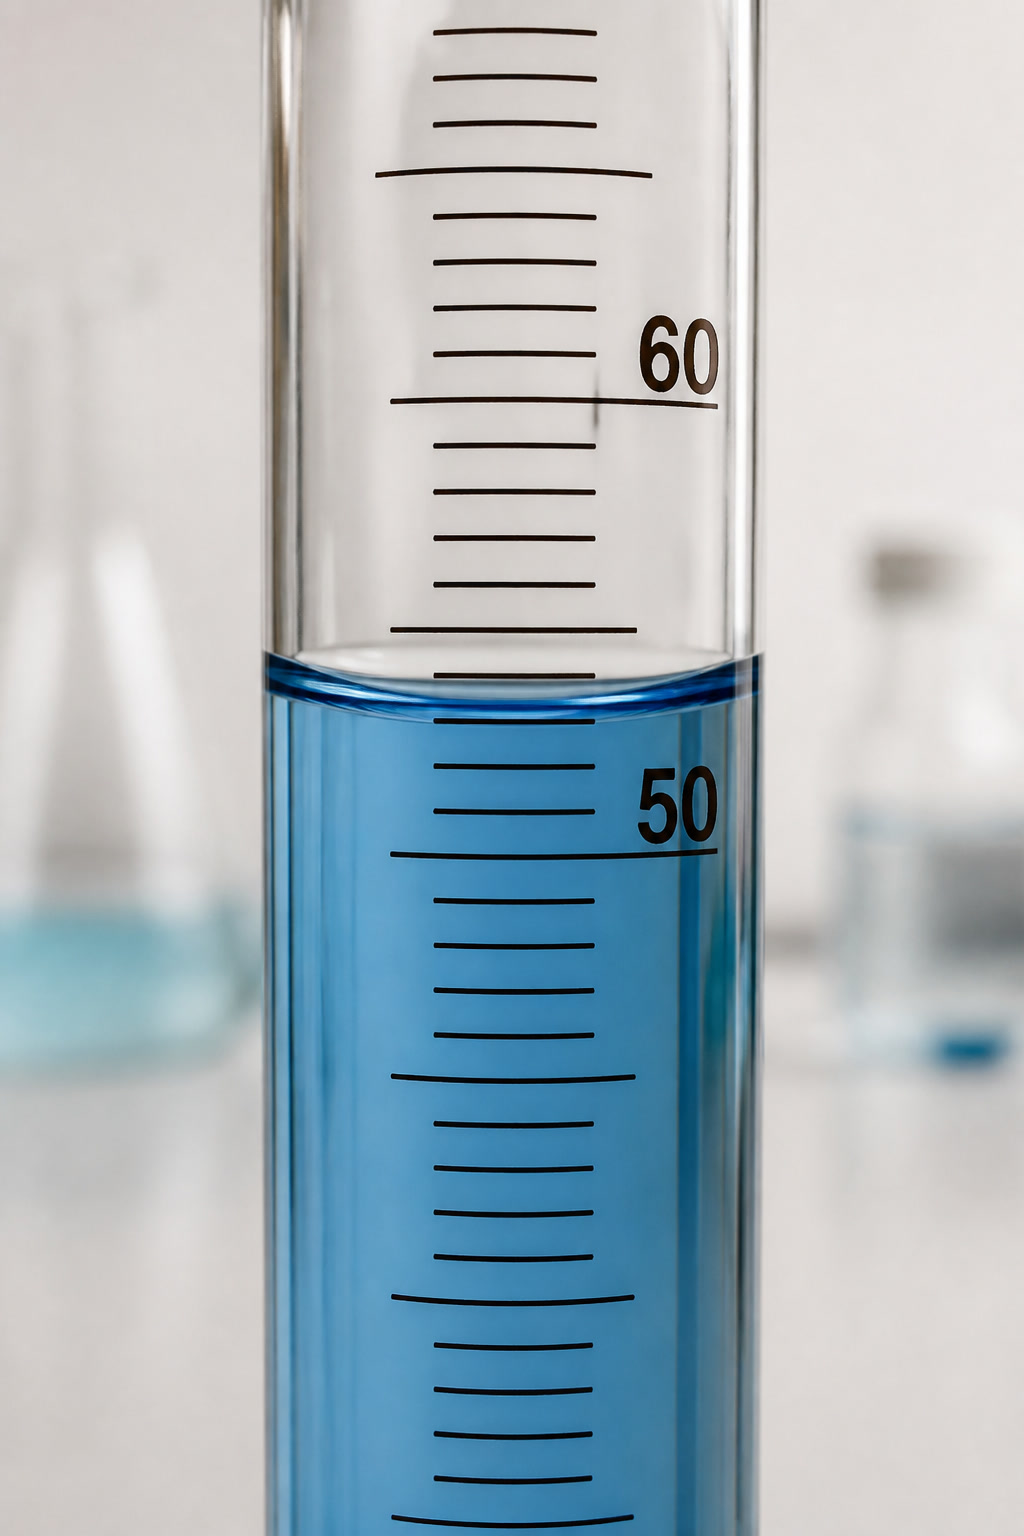
\includegraphics[width=0.3\linewidth]{images/book1/ai/g6-volume-cylinder.jpg}

{\small पास से देखा गया \omterm{met:g6:mass-and-volume:cylinder}{नवचंद्रक}: मोड़ के सपाट बीच वाले हिस्से को, आँख उसी की ऊँचाई पर रखकर पढ़ो।}
\end{omfigure}

\section{ठोसों को मापना --- गँठीले ठोसों को भी}

ईंट जैसे \omterm{def:g3:solids-liquids-gases:solid}{ठोस} रूलर के आगे हथियार डाल देते हैं: लंबाई गुणा चौड़ाई गुणा
ऊँचाई से उनका \omterm{def:g6:mass-and-volume:volume}{आयतन} \unit{cm^3} में मिल जाता है, जैसा तुम्हारे गणित के
पाठ्यक्रम ने दिखाया था। पर किसी कंकड़, चाबी या आलूबुख़ारे का क्या? किसी
गाँठदार टुकड़े पर रूलर बैठता ही नहीं। इसका उत्तर दो हज़ार साल पुराना
है, और वह नहाने के टब से निकला था।

\begin{proposition}[विस्थापन]\label{prop:g6:mass-and-volume:displacement}
पानी के भीतर पूरी तरह डुबोया गया \omterm{def:g3:solids-liquids-gases:solid}{ठोस} ठीक अपने ही \omterm{def:g6:mass-and-volume:volume}{आयतन} जितना पानी
हटाता है --- यानी विस्थापित करता है। पानी के तल का उठना उस घुसपैठिये
का माप है: गँठीला हो या चिकना, पानी उसके हर गड्ढे और हर उभार के अनुसार
ढल जाता है।
\end{proposition}

\begin{method}[पानी के उठने से आयतन]\label{met:g6:mass-and-volume:rise}
\begin{enumerate}
  \item मापक बेलन में पानी डालो --- इतना कि वस्तु डूब सके --- और
        \omterm{def:g6:mass-and-volume:volume}{आयतन} पढ़ो: मान लो \qty{120}{mL};
  \item वस्तु से एक धागा बाँधो और उसे धीरे-धीरे तब तक नीचे उतारो जब
        तक वह पूरी तरह डूब न जाए, बिना छपाक किए और बिना दीवारें
        छुए;
  \item फिर पढ़ो: मान लो \qty{145}{mL};
  \item घटाओ: $145 - 120 = 25$ --- वस्तु का \omterm{def:g6:mass-and-volume:volume}{आयतन} \qty{25}{cm^3} है
        (उठने के मिलीलीटर और पत्थर के \omterm{def:g2:measuring-length:units}{सेंटीमीटर} वाले घन: एक ही
        बात)।
\end{enumerate}
\end{method}

\begin{omfigure}
\begin{tikzpicture}[scale=0.85]
  \draw[thick] (0.8,0) -- (0.8,3.6) (2.6,0) -- (2.6,3.6)
    (0.8,0) -- (2.6,0);
  \fill[omDef, opacity=0.2] (0.8,0.05) rectangle (2.6,2.0);
  \draw[omDef, very thick] (0.8,2.0) -- (2.6,2.0);
  \node[right, font=\footnotesize] at (2.7,2.0) {120};
  \node[below, font=\small] at (1.7,-0.3) {पहले};
  \draw[thick] (6.2,0) -- (6.2,3.6) (8.0,0) -- (8.0,3.6)
    (6.2,0) -- (8.0,0);
  \fill[omDef, opacity=0.2] (6.2,0.05) rectangle (8.0,2.42);
  \draw[omDef, very thick] (6.2,2.42) -- (8.0,2.42);
  \node[right, font=\footnotesize] at (8.1,2.42) {145};
  \draw (7.1,3.6) -- (7.1,1.0);
  \fill[omExo] (7.1,0.75) ellipse (0.4 and 0.3);
  \node[below, font=\small] at (7.1,-0.3)
    {बाद में: कंकड़, पूरी तरह डूबा हुआ};
  \draw[-Stealth, omThm, thick] (4.0,2.0) -- (5.6,2.35);
  \node[below, font=\small, omThm] at (4.8,1.9)
    {उठान: \qty{25}{mL}};
\end{tikzpicture}

{\small उठान वाली विधि: पानी ठीक कंकड़ के \omterm{def:g6:mass-and-volume:volume}{आयतन} जितना चढ़ता है ---
$145 - 120 = \qty{25}{cm^3}$ का कंकड़।}
\end{omfigure}

\begin{example}[नहाने के टब में मुकुट]\label{ex:g6:mass-and-volume:archimedes}
पुरानी कहानी: एक राजा को शक हुआ कि उसके सुनार ने राजसी मुकुट के सोने
में चाँदी मिला दी है, और उसने वैज्ञानिक आर्किमिडीज़ से कहा कि मुकुट को
नुक़सान पहुँचाए बिना यह पता लगाओ। भरे हुए टब में पैर रखते ही आर्किमिडीज़
ने पानी को किनारे से छलककर बाहर गिरते देखा --- और उसी पल समझ लिया कि
वह छलका हुआ पानी उसके अपने शरीर का \omterm{def:g6:mass-and-volume:volume}{आयतन} नाप रहा है, गाँठों-उभारों
समेत। किंवदंती कहती है कि वह ``यूरेका!'' चिल्लाता हुआ गलियों में दौड़
पड़ा --- \emph{मैंने पा लिया!} मुकुट के \omterm{def:g6:mass-and-volume:volume}{आयतन} ने धोखाधड़ी का पर्दाफ़ाश
कैसे किया, इसके लिए एक और विचार चाहिए, जो दो अध्याय आगे है; टब ने तो
उसे \emph{किसी भी चीज़} का \omterm{def:g6:mass-and-volume:volume}{आयतन} दे दिया।
\end{example}

\section{द्रव्यमान और आयतन अलग-अलग उत्तर हैं}

\begin{example}[वही आयतन, अलग द्रव्यमान]\label{ex:g6:mass-and-volume:different}
एक जैसे \qty{25}{cL} वाले दो गिलास भरो, एक पानी से और एक शहद से, और
उन्हें तौलो (गिलासों का \omterm{def:g4:weight-and-mass:weight}{भार} घटाकर): शहद वाला गिलास ठीक उसी स्थान में
साफ़ तौर पर ज़्यादा \omterm{def:g3:measuring-mass:units}{ग्राम} रखता है। \omterm{def:g6:mass-and-volume:volume}{आयतन} वही, \omterm{def:g3:measuring-mass:mass}{द्रव्यमान} अलग। और एक \omterm{def:g6:mass-and-volume:volume}{लीटर}
\omterm{def:g2:air-around-us:air}{हवा} का \omterm{def:g4:weight-and-mass:weight}{भार} बमुश्किल एक \omterm{def:g3:measuring-mass:units}{ग्राम} से ज़्यादा होता है, जबकि उसी जगह में एक
\omterm{def:g6:mass-and-volume:volume}{लीटर} पानी का \omterm{def:g4:weight-and-mass:weight}{भार} पूरा एक \omterm{def:g3:measuring-mass:units}{किलोग्राम}। स्थान और पदार्थ सचमुच अलग-अलग
मुनीम हैं --- इस बात को कसकर पकड़े रखो: इसी साल के आख़िरी अध्याय में यह
नाम सहित एक नियम बन जाएगी।
\end{example}

\begin{remark}[उसे तौलना जो अकेला खड़ा नहीं हो सकता]\label{rem:g6:mass-and-volume:tare}
आटे को उसके कटोरे के बिना कैसे तौलें? आजकल की तुलाओं में इसके लिए एक
बटन होता है: ख़ाली कटोरा पलड़े पर रखो, बटन दबाओ --- पटल शून्य पर लौट
आता है --- फिर आटा डालो: अब \omterm{def:g3:levers-and-scales:scale}{तुला} अकेले आटे की ख़बर देती है। इस \omterm{def:g5:speed-distance-time:speed}{चाल} को
\emph{टेयरिंग} कहते हैं। बटन न हो तो दो बार तौलो और घटा लो:
कटोरा-सहित-आटा घटा ख़ाली कटोरा। दोनों तरह यह वही निष्पक्ष-शुरुआत वाला
नियम है: ईमानदार शून्य से शुरू करो।
\end{remark}

\section{अभ्यास}

\begin{exercise}[$\star$]\label{exo:g6:mass-and-volume:1}
\omterm{def:g6:mass-and-volume:volume}{आयतन} किस सवाल का उत्तर देता है, और \omterm{def:g3:measuring-mass:mass}{द्रव्यमान} किस सवाल का? हर एक के
दोनों मुख्य \omterm{def:g6:measurement-in-science:measuring}{मात्रक} बताओ।
\end{exercise}

\begin{exercise}[$\star$]\label{exo:g6:mass-and-volume:2}
बदलो: \qty{2}{L} को \unit{cm^3} में; \ \qty{350}{mL} को
\unit{cm^3} में; \ \qty{1500}{cm^3} को \omterm{def:g6:mass-and-volume:volume}{लीटर} में; \ आधा \omterm{def:g6:mass-and-volume:volume}{लीटर}
मिलीलीटर में।
\end{exercise}

\begin{exercise}[$\star$]\label{exo:g6:mass-and-volume:3}
मापक बेलन को मेज़ पर रखकर, आँख के बराबर, और \omterm{met:g6:mass-and-volume:cylinder}{नवचंद्रक} के सबसे नीचे से
क्यों पढ़ना चाहिए? हर नियम किस ग़लती से बचाता है?
\end{exercise}

\begin{exercise}[$\star$]\label{exo:g6:mass-and-volume:4}
एक बेलन \qty{200}{mL} दिखाता है; उसमें आलूबुख़ारा उतारने पर वह
\qty{265}{mL} दिखाता है। आलूबुख़ारे का \omterm{def:g6:mass-and-volume:volume}{आयतन} \unit{cm^3} में कितना है?
\end{exercise}

\begin{exercise}[$\star$]\label{exo:g6:mass-and-volume:5}
जिस गँठीले कंकड़ को कोई रूलर माप ही नहीं सकता था, उसके लिए भी उठान
वाली विधि क्यों काम कर जाती है? कौन-सी प्रतिज्ञप्ति उत्तर देती है?
\end{exercise}

\begin{exercise}[$\star$]\label{exo:g6:mass-and-volume:6}
ईंट जैसी एक रबड़ \qty{5}{cm} गुणा \qty{2}{cm} गुणा \qty{1}{cm} की
है। उसका \omterm{def:g6:mass-and-volume:volume}{आयतन}? जाँच की योजना: उठान वाली विधि से इसकी पुष्टि कैसे
करोगे?
\end{exercise}

\begin{exercise}[$\star$]\label{exo:g6:mass-and-volume:7}
चावल तौलने के लिए: ख़ाली कटोरा \qty{280}{g}; चावल सहित कटोरा
\qty{745}{g}। चावल कितना है? यही काम एक ही क़दम में कौन-सा बटन कर
देता है?
\end{exercise}

\begin{exercise}[$\star$]\label{exo:g6:mass-and-volume:8}
\omterm{def:g6:mass-and-volume:volume}{आयतन} किसका ज़्यादा है, एक \omterm{def:g3:measuring-mass:units}{किलोग्राम} पंखों का या एक \omterm{def:g3:measuring-mass:units}{किलोग्राम} लोहे का?
और \omterm{def:g3:measuring-mass:mass}{द्रव्यमान} किसका ज़्यादा है? (दोनों उत्तर ध्यान से दो।)
\end{exercise}

\begin{exercise}[$\star\star$]\label{exo:g6:mass-and-volume:9}
कॉर्क के लिए उठान वाली विधि नाकाम रहती है: वह तैर जाता है। ऐसा हल
सुझाओ जो फिर भी बेलन का ही उपयोग करे --- और बताओ कि अगर तुम्हारे हल
में कोई सहायक वस्तु लगे तो क्या घटाना पड़ेगा।
\end{exercise}

\begin{exercise}[$\star\star$]\label{exo:g6:mass-and-volume:10}
रस के डिब्बे पर \qty{1}{L} लिखा है। उँडेलने पर वह \qty{250}{mL} का
गिलास तीन बार भर देता है, और चौथा गिलास सिर्फ़ \qty{200}{mL} के
निशान तक। क्या दावा ईमानदार था? कितने से चूका?
\end{exercise}

\begin{exercise}[$\star\star$]\label{exo:g6:mass-and-volume:11}
\qty{80.0}{mL} दिखाते बेलन में एक हार उतारा जाता है; पानी
\qty{83.5}{mL} तक चढ़ जाता है। जौहरी दावा करता है कि हार में
\qty{5}{cm^3} सोना है। क्या यह दावा सच हो सकता है? पानी ने ठीक-ठीक
क्या मापा?
\end{exercise}

\begin{exercise}[$\star\star\star$]\label{exo:g6:mass-and-volume:12}
ख़ुद \cref{prop:g6:mass-and-volume:displacement} की जाँच के लिए
नहाने के टब जैसी कोई परीक्षा बनाओ, और उसमें ईंट जैसी वह वस्तु काम में
लो जिसका \omterm{def:g6:mass-and-volume:volume}{आयतन} रूलर पहले से जानता है। क़दम बताओ, $4 \times 3 \times 2$
\omterm{def:g2:measuring-length:units}{सेंटीमीटर} वाले गुटके को \qty{150}{mL} में उतारने पर बेलन के दोनों
पाठों का अंदाज़ा लगाओ, और यह भी बताओ कि कौन-सा परिणाम उस प्रतिज्ञप्ति
को ग़लत साबित कर देता।
\end{exercise}

\section{समस्या: बग़ीचे में बोतल भरने का दिन}

\begin{problem}[{सप्ताहांत समस्या --- बग़ीचे में रस निकालने का दिन;
लीटरों से बोतलों तक, पेटियों से तराज़ू तक; और जग में गिरा कंकड़}]\label{pb:g6:mass-and-volume:1}
बग़ीचे में आज सेबों का रस निकाला जा रहा है, और हर मददगार को मापने का
कोई न कोई काम मिला है।

\medskip\noindent\textbf{भाग I --- लीटरों में रस।}
मशीन ने \qty{20}{L} का एक पीपा भर दिया है।
\begin{enumerate}
  \item \qty{20}{L} कितने \omterm{def:g6:mass-and-volume:volume}{घन सेंटीमीटर} हुए?
  \item रस \qty{75}{cL} की बोतलों में भरा जाता है। पीपे से कितनी
        \emph{पूरी} बोतलें बनती हैं?
  \item आख़िरी पूरी बोतल के बाद कितना रस बचता है, सेंटीलीटर में?
  \item बचा हुआ रस \qty{25}{cL} के गिलासों में उँडेला जाता है। वह
        कितने गिलास भरता है?
\end{enumerate}

\medskip\noindent\textbf{भाग II --- तराज़ू पर पेटियाँ।}
\begin{enumerate}[resume]
  \item ख़ाली बोतल का \omterm{def:g3:measuring-mass:mass}{द्रव्यमान} \qty{450}{g} है। भाग I की मदद से
        बताओ कि एक पूरी बोतल के रस का \omterm{def:g3:measuring-mass:mass}{द्रव्यमान} कितना है, अगर एक
        \omterm{def:g6:mass-and-volume:volume}{लीटर} रस का \omterm{def:g3:measuring-mass:mass}{द्रव्यमान} लगभग \qty{1}{kg} हो। (\omterm{def:g3:measuring-mass:units}{ग्राम} में काम
        करो।)
  \item तो एक पूरी बोतल का कुल \omterm{def:g4:weight-and-mass:weight}{भार} कितना हुआ?
  \item लकड़ी की एक पेटी ख़ाली हालत में \qty{2}{kg} की है और उसमें
        छह पूरी बोतलें आती हैं। लदी हुई पेटी का कुल \omterm{def:g3:measuring-mass:mass}{द्रव्यमान}?
  \item वैन \qty{200}{kg} तक की पेटियाँ ढो सकती है। वह कितनी लदी
        हुई पेटियाँ ले जा सकती है? (सिर्फ़ पूरी पेटियाँ।)
\end{enumerate}

\medskip\noindent\textbf{भाग III --- जग में कंकड़।}
नन्हा टॉम रस से लबालब भरे \qty{1}{L} के जग में एक कंकड़ गिरा देता है,
और रस छलककर मेज़ पर गिर जाता है।
\begin{enumerate}[resume]
  \item पोंछकर इकट्ठा किया गया छलका रस \qty{40}{mL} निकलता है। इस
        छलकने ने कंकड़ के बारे में क्या माप दिया, और किस
        प्रतिज्ञप्ति से?
  \item कंकड़ निकाल लेने के बाद जग में कितना रस बचता है?
  \item टॉम विरोध करता है: ``कंकड़ तो छोटा-सा है --- देखो, मेरी
        मुट्ठी में छिप जाता है!'' उसकी बहन मापक बेलन से जवाब देती
        है: वह कंकड़ को \qty{100}{mL} पानी में डालती है। कौन-सा पाठ
        साबित कर देगा कि छलके रस ने सच कहा था?
  \item अतिरिक्त हिसाब: रसोई की तराज़ू पर कंकड़ \qty{104}{g} का
        निकलता है। कोई नया विचार लाए बिना, क्या तुम अभी बता सकते हो
        कि \emph{बराबर जगह घेरने पर} कंकड़ का पदार्थ रस के पदार्थ से
        भारी है या हल्का? \qty{40}{cm^3} में \qty{104}{g} कंकड़ की
        तुलना उस \omterm{def:g3:measuring-mass:mass}{द्रव्यमान} से करो जो उन्हीं \qty{40}{cm^3} में रस का
        होता --- और अपना निष्कर्ष घनत्व वाले अध्याय के लिए गरम रखो।
\end{enumerate}
\end{problem}
